% Copyright (c) 2022 Tobias Briones. All rights reserved.
% SPDX-License-Identifier: CC-BY-SA-4.0
%
% This source code is part of
% https://github.com/tobiasbriones/cp-unah-is911-microprocessors and is
% licensed under the Creative Commons Attribution Share Alike 4.0
% International License found in the LICENSE file in the root
% directory of this source tree or at https://spdx.org/licenses/CC-BY-SA-4.0

\documentclass{article}
\usepackage{preamble}
\usepackage{amsmath}

\title{LAB 5: GAL16v8 Simulación de Circuito}
\author{Tobias Briones \bigbreak tobias.briones@unah.hn}
\date{Septiembre 2021}

\begin{document}

    \makeatletter
    \begin{titlepage}
        \begin{center}
            
\includegraphics[width=0.3\linewidth]{images/logo-unah}\\[4ex]
            {\huge \bfseries \@title
            \vspace{1cm}}\\[2ex]
            {\LARGE \@author}\\[50ex]

            {\large
            Universidad Nacional Autónoma de Honduras\\
            Ingeniería de Sistemas\\
            I PAC 2022\\
            IS911-MICROPROCESADORES
            }\\[2ex]

            {\large \today}
        \end{center}
    \end{titlepage}
    \makeatother
    \thispagestyle{empty}
    \newpage

    \import{}{footer}

    \section{Objetivo}\label{sec:objetivo}

    Crear una simulación del circuito dado en GAL16v8 y Proteus.

    \subsection{Objetivos Específicos}\label{subsec:objetivos-específicos}

    \begin{itemize}
        \item Entender la tarjeta GAL16v8.
        \item Convertir el diagrama lógico en una fórmula.
        \item Implementar la simulación del circuito en Proteus.
    \end{itemize}

    \section{Marco Teórico}\label{sec:marco-teórico}

    Los dispositivos lógicos programables (DLP) o programmable logic devices
    (PLD) son dispositivos de hardware que no tienen una funcionalidad
    predeterminada de fábrica como las compuertas lógicas. Esta funcionalidad
    es dada por el programador.

    \subsection{Definiciones}

    \begin{quote}
        Un dispositivo lógico programable (PLD) es un componente electrónico
        utilizado para construir circuitos digitales reconfigurables. A
        diferencia de la lógica digital construida utilizando puertas lógicas
        discretas con funciones fijas, un PLD tiene una función indefinida en
        el momento de la fabricación.\\ \footnotesize
        Fuente: \textit{Wikipedia} $\mid$ Programmable logic device
        \cite{wikipedia-pld-2022} (traducido de inglés a español)
    \end{quote}

    Hay muchas formas de utilizarlos, entre ellas \cite{wikipedia-pld-2022}:

    \begin{itemize}
        \item Simple Programmable Logic Devices (SPLDs).
        \item Complex Programmable Logic Devices (CPLDs).
        \item Field-Programmable Gate Arrays (FPGAs).
    \end{itemize}

    Los GALs (cuales nos interesa) son útiles para prototipos y una mejora de
    los PAL. GAL significa \say{Dispositivo de Lógica de Arreglo Genérico}. Y
    su forma física es como la siguiente:

    \begin{figure}[H]
        \centering
        \includegraphics[width=0.5\paperwidth]{images/lattice-gal-16v8}
        \caption{GAL16V8}\footnotesize
        Fuente: \textit{Wikipedia} $\mid$  Programmable logic device
        \cite{wikipedia-pld-2022}. By Michael Holley - English Wikipedia,
        Public Domain, https://commons.wikimedia.org/w/index.php?curid=3146615.
    \end{figure}

    \subsection{Características del GAL16V8}

    Las principales características de GAL16V8 son
    \cite{lattice-semiconductor-corp-2004}:

    \begin{itemize}
        \item Tecnología de alto rendimiento.
        \item $50\%$ a $75\%$ de reducción en potencia.
        \item PULL-UPS activos en todos los pins.
        \item Tecnología CELL $E^2$.
        \item Ocho marcoceldas de salida lógica.
        \item Precarga y reinicio de encendido para todos los registros.
        \item Aplicaciones como control de DMA, control de máquina de
        estados, proceso de gráficos de alta velocidad.
        \item Firma electrónica para identificación.
    \end{itemize}


    \begin{figure}[H]
        \centering
        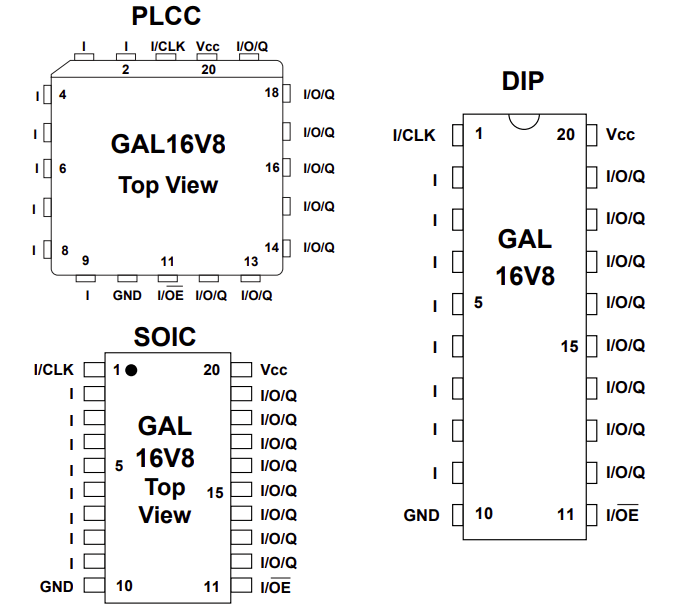
\includegraphics[width=0.5\paperwidth]{images/datasheet-gal16v8-pins}
        \caption{GAL16V8 Configuración de Pines}\footnotesize
        Fuente: \textit{ece-classes.usc.edu} $\mid$ GAL16V8 Data Sheet
        \cite{lattice-semiconductor-corp-2004} (bajo uso justo)
    \end{figure}

    Podemos hablar sobre otros detalles como las operaciones lógicas. Estas
    se definen como $(!, NOT)$, $(\&, AND)$, $(\#, OR)$, $(\$, XOR)$
    \cite{warneke-1998}.

    \bigbreak

    Por otro lado, la extensión de archivo que necesitamos, la cual contiene
    el mapa de fusible (código a simular) es el archivo con formato JED. Este
    es generado por CUPL y usado por el programador para quemar el chip
    \cite{warneke-1998}.

    \section{Procedimiento Experimental}\label{sec:procedimiento-experimental}

    \begin{figure}[H]
        \centering
        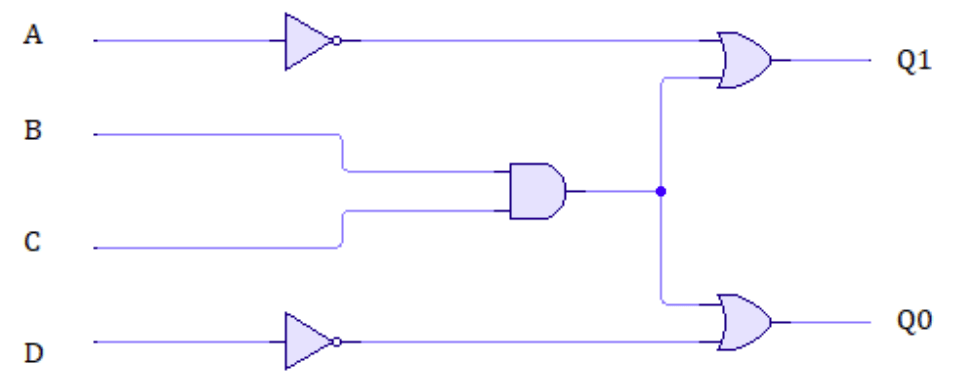
\includegraphics[width=0.5\paperwidth]{images/logic-circuit}
        \caption{Circuito Lógico}
    \end{figure}

    Este circuito combinacional tiene la siguiente ecuación:

    $$Q_1 = !A | (A \& B)$$

    $$Q_0 = !D | (B \& C)$$

    \subsection{Programa}

    Primero se debe instalar el software WinCUPL de
    \href{https://www.microchip.com/en-us/products/fpgas-and-plds/spld-cplds/pld-design-resources}{La descarga oficial}.
    Puede salir un mensaje de advertencia que no se puede descargar de forma
    segura.

    \begin{figure}[H]
        \centering
        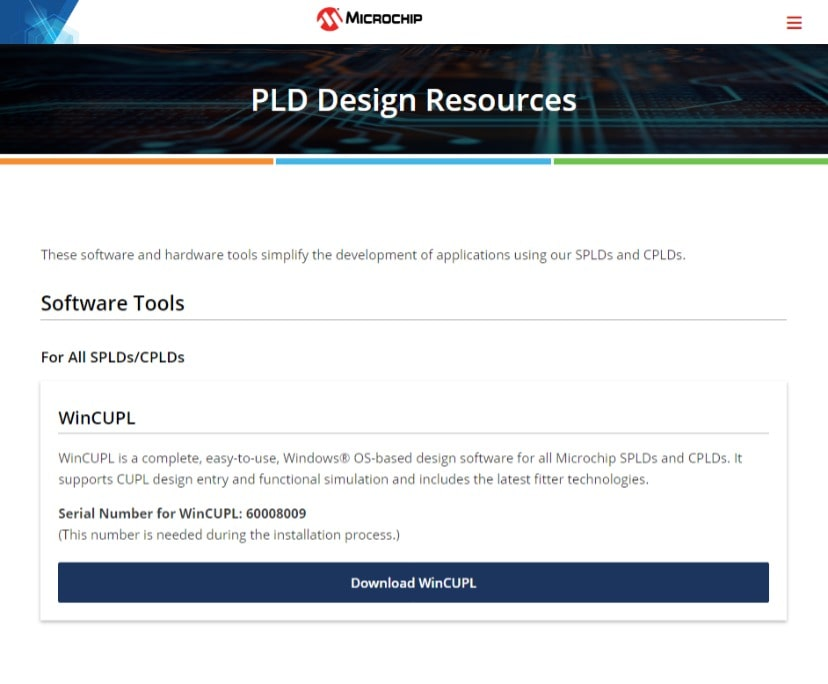
\includegraphics[width=0.5\paperwidth]{images/microchip.com-download-wincupl}
        \caption{Descarga de WinCUPL}
    \end{figure}

    El software es super anticuado (data de los años 80s), inseguro de
    descargar (el navegador no permite su descarga), y el binario no está
    firmado, por lo cual no es software de confianza pero es lo que hay. En
    la página de descarga se da un serial, con este se deberá ingresar al
    programa. Siendo así, se seguirán los siguientes pasos:

    \bigbreak

    Crear un nuevo proyecto, y agregar los siguientes datos

    \begin{figure}[H]
        \centering
        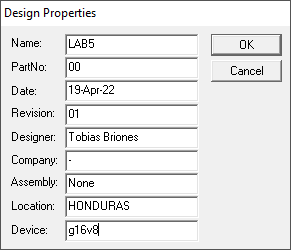
\includegraphics[width=0.3\paperwidth]{images/wincupl-design-properties}
        \caption{Descarga de WinCUPL}
    \end{figure}

    El campo Device debe contener la tarjeta que se va a emplear.

    \bigbreak

    A continuación, se ingresa la cantidad de entradas ($4$) y salidas ($2$)
    que se van a utilizar. El pinnodes no se utilizará por lo que se deja en
    $0$.

    \bigbreak

    En el programa, se definen las entradas primero, luego las salidas, y por
    último la lógica del programa para asignar las salidas el valor que se
    obtuvo en las fórmulas.

    \bigbreak

    Cabe destacar, que en el lenguaje CUPL, además de lo que se verá a
    continuación, la sintaxis cambia un poco, utilizando ! para NOT, \# para
    OR, y \& para AND.

    \begin{figure}[H]
        \centering
        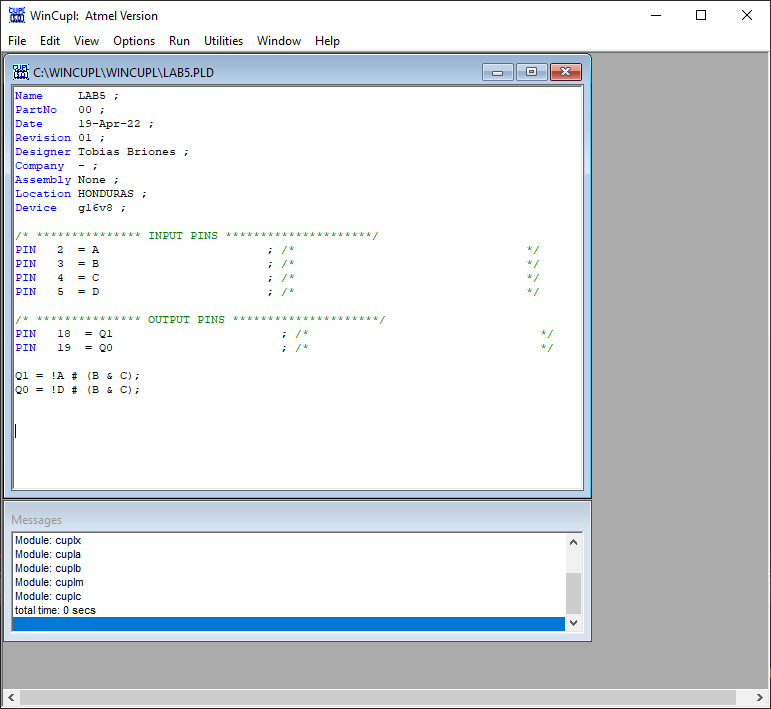
\includegraphics[width=0.5\paperwidth]{images/wincupl-program}
        \caption{Programa CUPL}
    \end{figure}

    Por lo que se procede a guardar y compilar el código con F9. El archivo
    binario se encontrará el directorio de instalación de WinCUPL -> WinCUPL
    -> LAB5.jed.

    \subsection{Simulación}

    Se abre un nuevo proyecto en Proteus, y se agregan los siguientes
    dispositivos:

    \begin{itemize}
        \item AM16V8
        \item LED-AQUA
        \item RES
        \item SW-SPST
    \end{itemize}

    \begin{figure}[H]
        \centering
        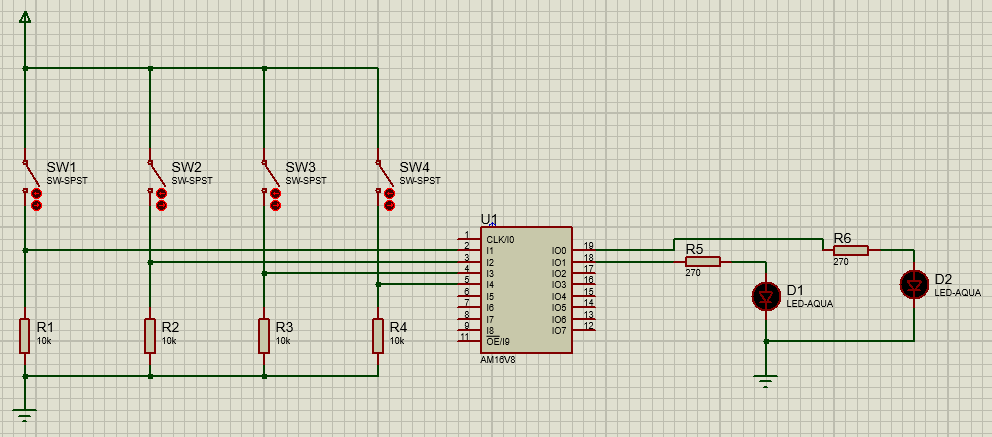
\includegraphics[width=0.5\paperwidth]{images/proteus-sim-circuit}
        \caption{Circuito para la Simulación}
    \end{figure}

    Para agregar el mapa de fusible, hacer doble click en el integrado, y
    seleccionar el mapa de fusible, o archivo .jed.

    \section{Análisis de Resultados}\label{sec:análisis-de-resultados}

    Corriendo la simulación, con los valores siguientes se obtuvieron:

    \bigbreak

    Si todos son cero $\implies$ $Q_1 = 1$ y $Q_0 = 1$.

    \begin{figure}[H]
        \centering
        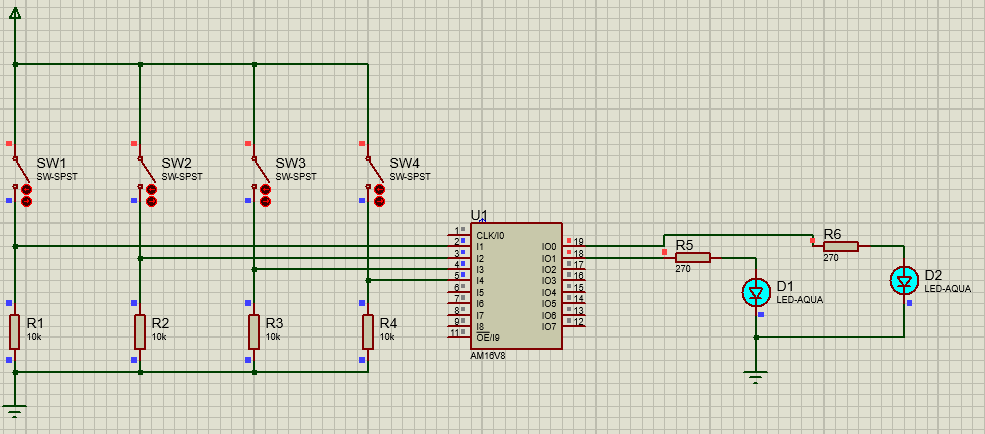
\includegraphics[width=0.5\paperwidth]{images/proteus-sim-1}
        \caption{Simulación 1}
    \end{figure}

    \bigbreak

    Si se tiene $0001$ $\implies$ $Q_1 = 1$ y $Q_0 = 0$.

    \begin{figure}[H]
        \centering
        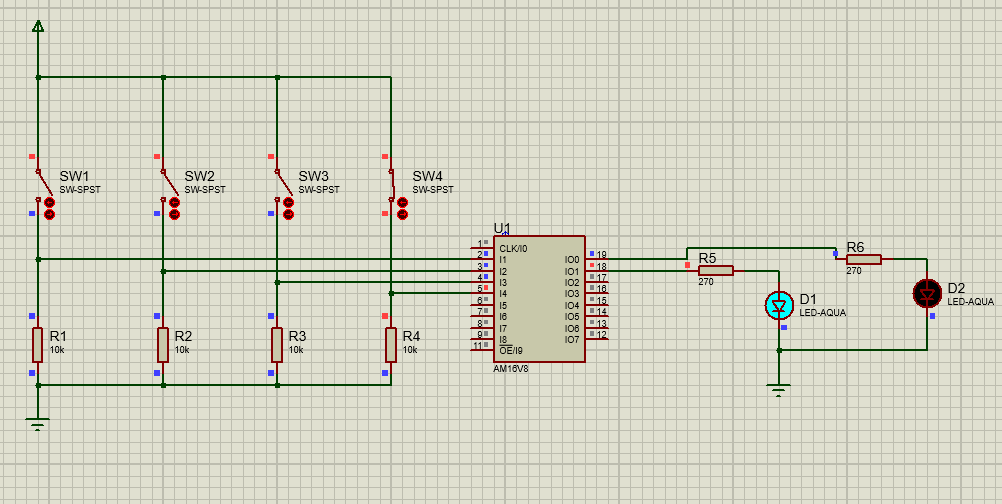
\includegraphics[width=0.5\paperwidth]{images/proteus-sim-2}
        \caption{Simulación 2}
    \end{figure}

    \bigbreak

    Si se tiene $0011$ $\implies$ $Q_1 = 1$ y $Q_0 = 0$.

    \begin{figure}[H]
        \centering
        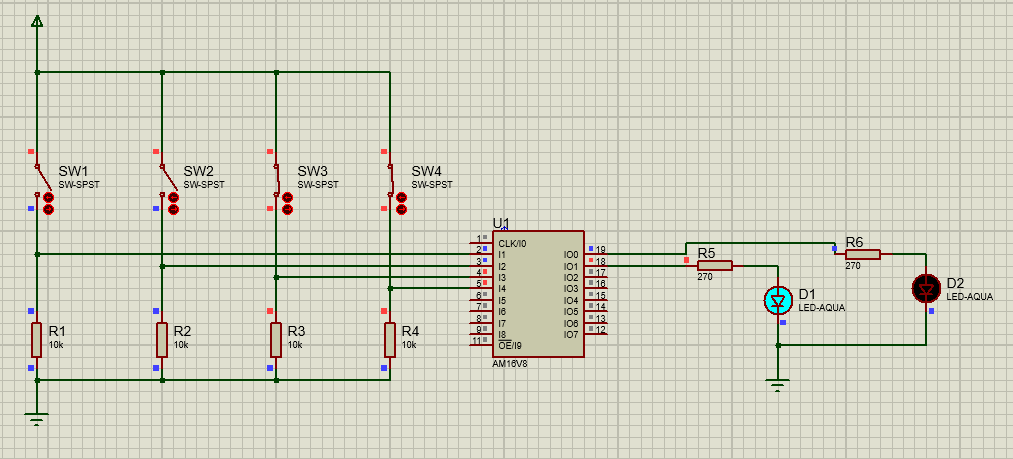
\includegraphics[width=0.5\paperwidth]{images/proteus-sim-3}
        \caption{Simulación 3}
    \end{figure}

    De igual forma, se pudo terminar de comprobar la funcionalidad del
    programa con los valores restantes de la tabla de verdad del problema
    resuelto.

    \section{Conclusión}\label{sec:conclusion}

    Se instaló el software WinCUPL para compilar el programa del problema
    propuesto. Se convirtió el circuito lógico a una tabla de verdad o
    ecuación lógica. Se simuló el programa en Proteus y se verificó su
    funcionamiento normal.

    \printbibliography

\end{document}
